\documentclass[11pt]{article}

\usepackage[margin=1in]{geometry}
\usepackage{graphicx}
\usepackage{amsmath}
\usepackage[hidelinks]{hyperref}
\usepackage{authblk}
\usepackage{caption}
\captionsetup{labelfont=bf,font=small}
\graphicspath{{figures/}}
\renewcommand{\familydefault}{\sfdefault}

\title{When does ESM3 fuse its modalities? A geometry-first atlas of the
multimodal residual stream}
\author[1]{Jacob L. Steenwyk}
\affil[1]{\small Affiliation to be completed}
\date{}

\begin{document}
\maketitle

\begin{abstract}
\noindent ESM3 ingests a protein through several channels at once, including
amino-acid sequence, three-dimensional structure, secondary structure (SS8),
solvent accessibility (SASA), and discrete functional annotations, summing their
embeddings into a single residual stream. Whether these modalities occupy separate
subspaces, and at what depth they fuse, has not been characterised. The present
analysis runs \texttt{esm3-sm-open-v1} once per modality in isolation and applies
representational-similarity analysis across all 48 layers. The four physical
modalities (sequence, structure, SS8, SASA) begin in distinct subspaces, remain
maximally separated through roughly the first half of the network, and then fuse
into a shared low-dimensional subspace between layers 25 and 35. The fusion is
ordered. The structure-derived modalities (structure, SS8, SASA) are mutually
aligned from the input, whereas sequence joins last, after layer 28. The
functional-annotation modality never fuses. It remains representationally
orthogonal to the physical modalities at every layer, and this orthogonality holds
whether the annotation is supplied whole-protein or per-residue, which identifies
it as a content-driven separation rather than a tokenisation artifact. The fusion
is a learned property, absent in a randomly initialised model of the same
architecture, holds at the residue level below the mean-pool, and reorganises
variance, converting between-condition variance into within-condition variance
while the stream never approaches isotropy. Fusion depth is independent of protein
length but is delayed by structural disorder. The phenomenon is universal across
the tree of life. Across 5,555 proteins from 12 organisms spanning eukaryota,
bacteria, and archaea, every superkingdom, and every individual organism, reaches
peak modality fusion at the same network depth (layer 35).
\end{abstract}

\section{Introduction}

Multimodal protein language models such as ESM3 \cite{hayes2024} reason jointly over
sequence and structure. Each input modality has its own embedding table, and the
per-residue embeddings are summed before the transformer trunk. This architecture
raises a mechanistic question. The modalities may be kept in separate parts of the
representation, or the network may blend them, and if it blends them, the depth at
which it does so is unknown. Prior interpretability work on protein language models
has examined attention heads and learned features \cite{vig2021,rao2019,gujral2024,
cunningham2023}, but how the several input modalities of a multimodal model are
organised geometrically across depth has not been characterised.

The present analysis takes a geometry-first, descriptive approach. For each
protein, ESM3 runs once per modality in isolation, with all other modalities
masked, together with an all-modalities reference, and the residual stream is read
out at every layer. The resulting collection of per-(protein, modality, layer)
representations forms an atlas of how multimodal information is organised across
depth. Standard representational-geometry tools, namely silhouette score, linear
CKA, effective rank, and linear probes, characterise the atlas, supported by
several controls. This work is the first stage of a larger program. A companion
study \cite{steenwyk_companion} applies sparse autoencoders to ESM3 and ESM2 and,
among other results, reports that the sequence and sequence-plus-structure
representations of ESM3 converge between layers 28 and 38. The present analysis
extends that two-condition observation to a full multimodal atlas, characterising
the ordered fusion of the four physical modalities, the persistent orthogonality of
the functional channel, the universality of the pattern across the tree of life, and
a battery of controls; causal steering and sparse-autoencoder dictionaries are
developed in that companion work.

\section{Methods}

\paragraph{Model and modalities.} The model is \texttt{esm3-sm-open-v1}
\cite{hayes2024} (1.4 billion parameters, 48 transformer blocks, model dimension
1536). Six conditions are studied, comprising five single-modality inputs (sequence,
structure, SS8, SASA, and function) and an all-modalities condition in which every
modality is supplied jointly. Structure is provided as vector-quantised structure
tokens derived from coordinates, SS8 is computed by DSSP \cite{kabsch1983} and SASA
by the Shrake-Rupley algorithm \cite{shrake1973} from the structure, and function
is provided as whole-protein InterPro annotations \cite{paysanlafosse2023} filtered
to the 29{,}026-entry vocabulary of the ESM3 function tokeniser.

\paragraph{Datasets.} Three datasets were used, namely a 199-protein human pilot
for development, an 892-protein human set for the main results, and a 5,984-protein
set drawn from 12 organisms spanning eukaryota, bacteria, and archaea for the
universality test. Structures are AlphaFold-DB models of a single release
\cite{jumper2021,varadi2022}, SS8 and SASA are computed with DSSP (mkdssp 4.6.1, via
ESM's \texttt{ProteinChain}) \cite{kabsch1983}, and InterPro and Gene Ontology
annotations are taken from UniProt \cite{uniprot2023,paysanlafosse2023}. A
fourth dataset of 177 proteins backed by experimental (X-ray and cryo-EM) structures
from the RCSB replicates the main result with non-predicted coordinates.

\paragraph{Harvesting.} For each (protein, condition) pair, ESM3 runs one forward
pass and the residual stream is cached at all 48 layers, mean-pooled over residues
with the special tokens excluded. A 100-protein subset additionally stores
per-residue activations at seven layers for the pooling control.

\paragraph{Metrics.} Each layer is summarised by the silhouette score
\cite{rousseeuw1987} of the conditions (Euclidean, in the full 1536-dimensional
space), by the linear CKA of Kornblith et al. \cite{kornblith2019} between every
protein-aligned condition pair, by an integration index defined as the mean pairwise
CKA, by the effective rank \cite{roy2007} computed as the exponential of the entropy
of the covariance eigenspectrum for the whole cloud and for each condition, and by a
protein-grouped five-fold logistic probe of modality identity evaluated both in the
full space and in the top-3 PCA geometry.
Visualisations use PCA, fit per layer and in a shared basis across layers.

\paragraph{Controls.} The controls comprise a randomly initialised model whose
trunk and modality embeddings are reset while the structure encoder is preserved, a
per-residue replication, a subsampling-convergence analysis, label-permutation
nulls, and protein-bootstrap confidence intervals.

\section{Results}

\subsection{Physical modalities fuse sharply at mid-depth}

Condition separation, measured by silhouette score, rises from 0.32 at the input to
a maximum of 0.42 at layer 24, then falls to a minimum of 0.156 at layers 35 to 38,
with a partial re-separation at the final layers (Figure~\ref{fig:fig1}b). The
integration index moves inversely. The transition is sharp and localised, with a
knee near layer 25, rather than gradual. The accompanying joint-PCA projection
shows five separated clusters through layer 24 that collapse into one cloud by
layer 35 (Figure~\ref{fig:fig1}a).

\begin{figure}[t]
\centering
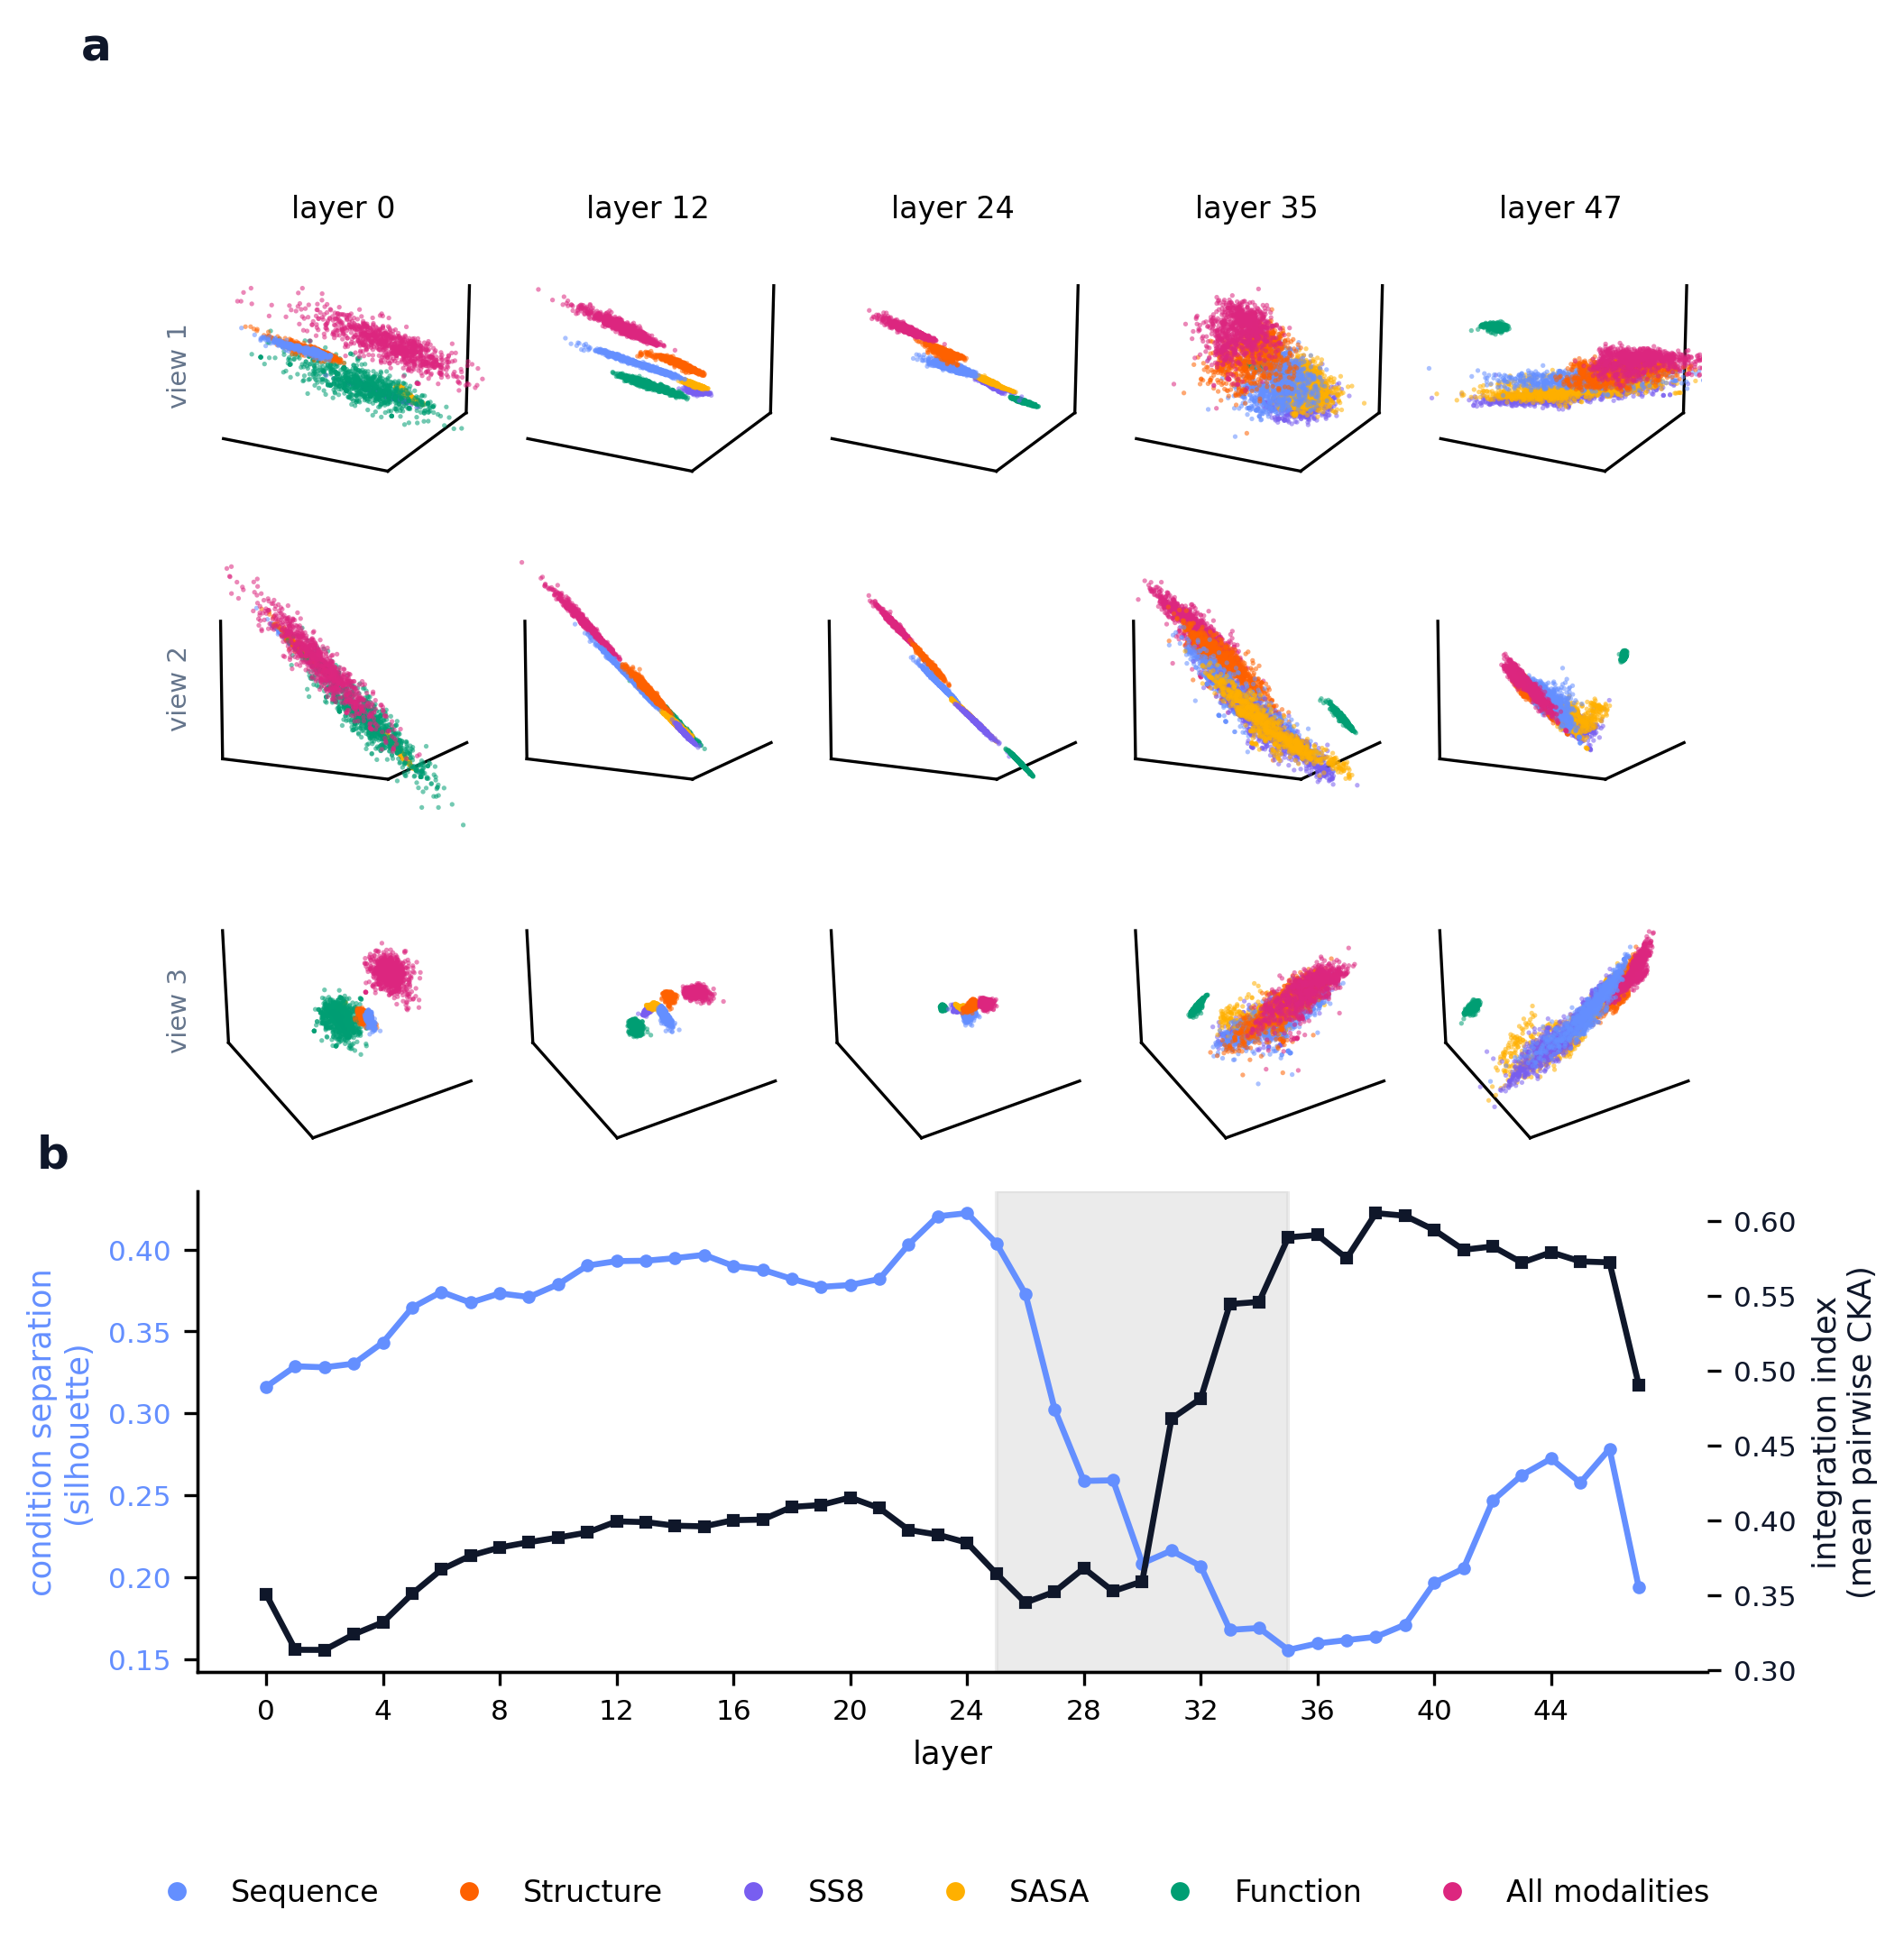
\includegraphics[width=\linewidth]{figure1.png}
\caption{Modality conditions occupy distinct subspaces early and fuse into a shared
subspace at mid-depth. (a) Mean-pooled residual-stream representations of 892 human
proteins under each single-modality condition, projected with a joint PCA fit
across all 48 layers and shown at five depths from three camera orientations
(rows), coloured by modality. The five
conditions form separated clusters through layer 24 and collapse into one cloud by
layer 35, while the functional-annotation condition (green) remains a distinct
island. (b) Across all 48 layers, condition separation (silhouette, left axis)
rises to a maximum of 0.42 at layer 24, then falls to a minimum of 0.156 at
layer 35, while the integration index (mean pairwise CKA, right axis) moves
inversely. The shaded band marks the fusion transition (layers 25 to 35).}
\label{fig:fig1}
\end{figure}

\subsection{The fusion is ordered, and sequence joins last}

Per-pair CKA shows that the structure-derived modalities (structure, SS8, and SASA)
are mutually aligned from layer 0, whereas every pairing that involves sequence
stays near a CKA of 0.2 until layer 28 and rises thereafter
(Figure~\ref{fig:fig2}a). Sequence, the one channel carrying information that cannot
be derived from the structure, integrates last.

\subsection{The functional-annotation modality never fuses}

Every pairing of the function condition with another condition stays near a CKA of
0.01 to 0.05 across all 48 layers, while structure reaches a CKA of about 0.99 with
the all-modalities reference. This orthogonality does not stem from a degenerate
representation, because the function cloud retains genuine cross-protein spread, with
an effective rank of 3.5 to 218 across layers. One alternative explanation is
granularity, because function is the only whole-protein modality whereas the
physical modalities vary residue by residue. To test this explanation, the
per-residue \texttt{residue\_annotation} modality of ESM3 was added, driven by
InterPro residue-site annotations available for 632 of the 892 proteins. Per-residue
functional annotation also stays largely orthogonal, with a CKA against the physical
modalities near 0.1 and a transient maximum near 0.5, never approaching the CKA of
about 0.99 that marks fusion (Figure~\ref{fig:fig2}b). Functional information is
therefore held in a separate subspace irrespective of granularity, a content-driven
separation.

\begin{figure}[t]
\centering
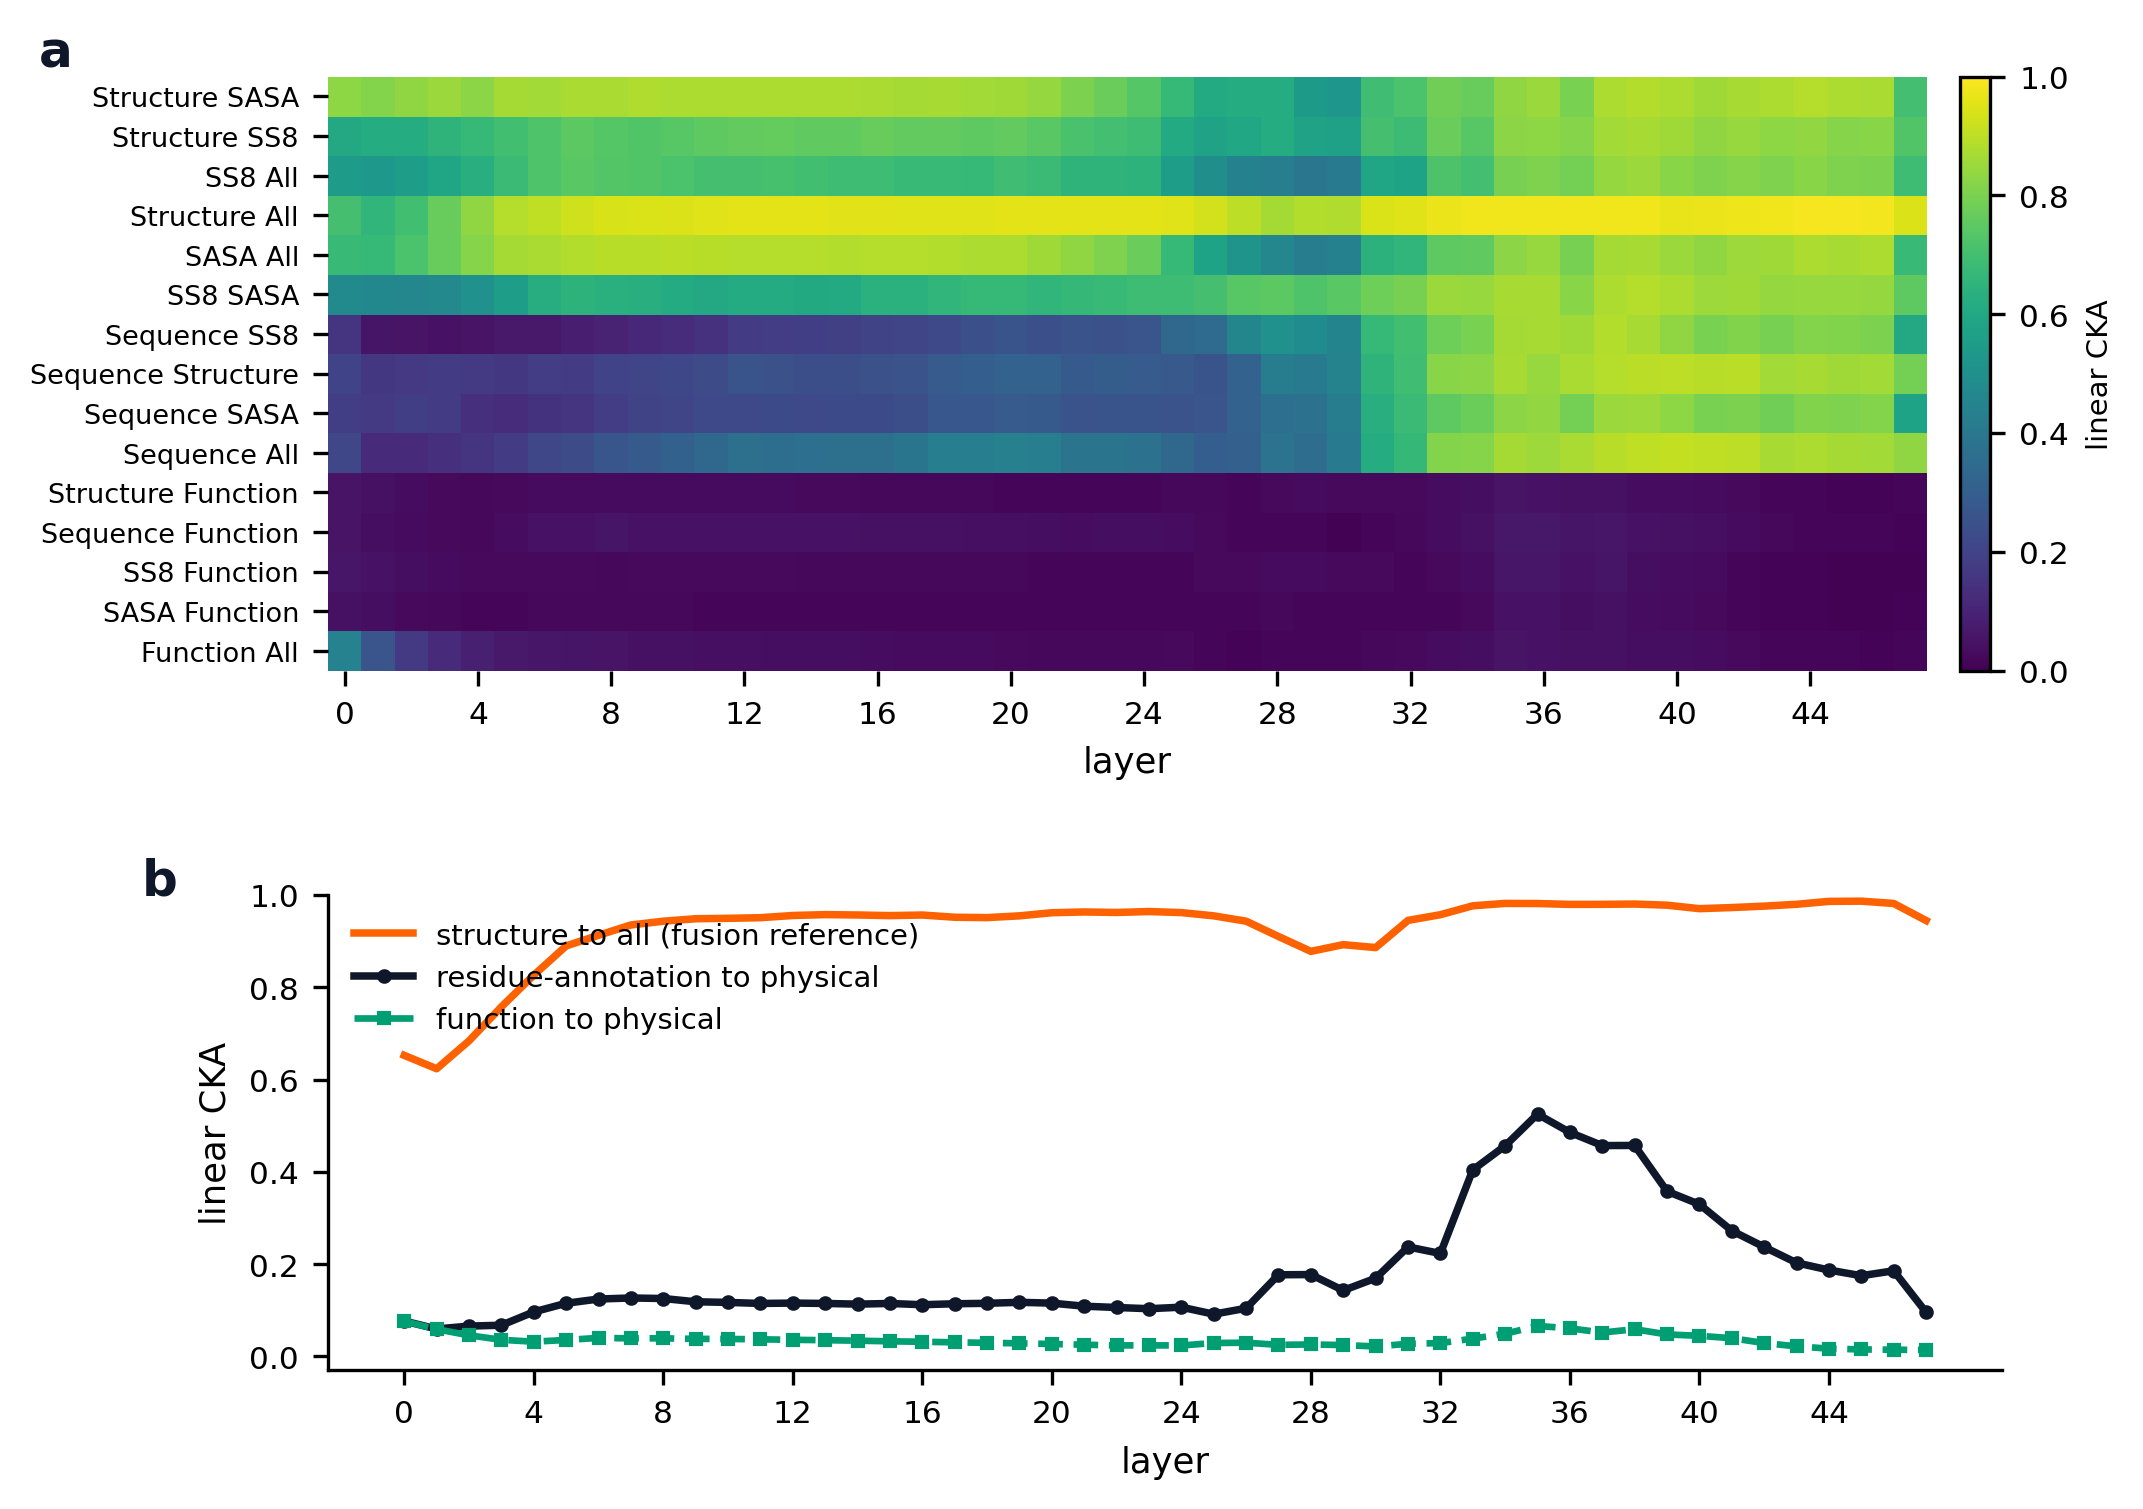
\includegraphics[width=\linewidth]{figure2.png}
\caption{Fusion of the physical modalities is ordered, and the functional channel
never joins. (a) Linear CKA between every condition pair at every layer, with rows
ordered by fusion onset (the first layer reaching a CKA of 0.5). The structure, SS8,
and SASA block is warm from layer 0, the sequence pairs warm only after layer 28,
and the five function pairs (bottom rows) stay near a CKA of 0.01 throughout.
(b) The whole-protein function track and the per-residue residue-annotation track
behave alike. Structure reaches a CKA of about 0.99 with the all-modalities
reference (orange), whereas residue-annotation (black) and function (green) both stay
below a CKA of 0.5 with the physical modalities.}
\label{fig:fig2}
\end{figure}

\subsection{The fusion is learned, not architectural}

A model with the same architecture but randomly initialised trunk and modality
embeddings, with the structure encoder preserved so that inputs remain meaningful,
shows no fusion. Condition separation stays near 0.62 and the integration index near
0.71 across all 48 layers, against the trained model's peak-then-collapse
(Figure~\ref{fig:fig3}a). Fusion is therefore a learned property and not a
consequence of summing modality embeddings.

\subsection{Fusion holds below the mean-pool}

Recomputed on residue-level representations of a 100-protein subset, the integration
index rises with depth from 0.19 to 0.59, mirroring the pooled curve
(Figure~\ref{fig:fig3}b). Fusion is not an averaging artifact.

\subsection{Fusion reorganises variance without approaching isotropy}

Effective rank of the whole cloud collapses to about 3 at the layer-24 separation
peak, then expands to about 85 of a possible 1536 in the fusion zone before
contracting, and the whole-cloud and per-condition ranks converge once the conditions
are fused (Figure~\ref{fig:fig3}c). Fusion therefore converts between-condition
variance into within-condition variance while the stream never approaches isotropy. A
logistic probe of modality identity reaches an accuracy of 1.0 in the full
1536-dimensional stream at every layer, which indicates that a thin additive identity
signal persists, whereas the same probe in the top-3 PCA geometry falls to about 0.68
in the fusion zone, driven mainly by SASA, even as the function condition stays
decodable throughout (Figure S3).

\begin{figure}[t]
\centering
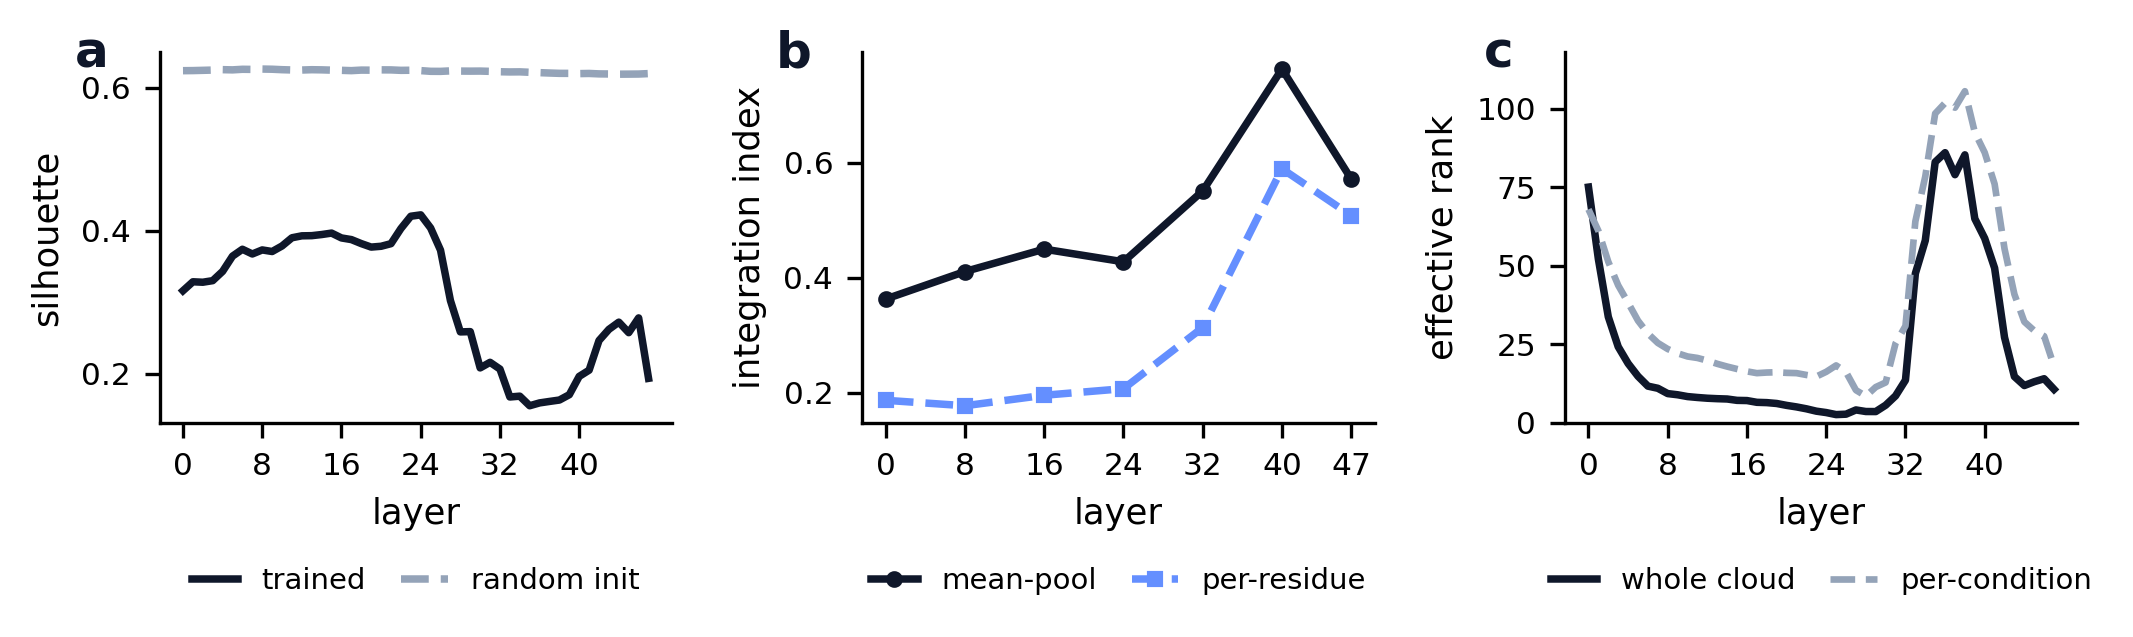
\includegraphics[width=\linewidth]{figure3.png}
\caption{The fusion is learned, holds below the mean-pool, and reorganises variance
without approaching isotropy. (a) A model with the same architecture but randomly
initialised weights shows no fusion, with condition separation near 0.62 at every
layer against the trained model's peak-then-collapse. (b) On residue-level
representations of a 100-protein subset, the integration index rises with depth
(0.19 to 0.59), mirroring the pooled curve. (c) Effective rank of the whole cloud
collapses to about 3 at the layer-24 separation peak, expands to about 85 of 1536 in
the fusion zone, then contracts, and the whole-cloud and per-condition ranks converge
once fused.}
\label{fig:fig3}
\end{figure}

\subsection{Fusion depth tracks secondary-structure content}

Across the 892 proteins, fusion-onset depth is independent of protein length
(Spearman r of $-0.04$, p of 0.26) but is delayed by structural disorder, with a
coil-fraction correlation of $+0.22$ ($p = 3 \times 10^{-11}$) and a helix-fraction
correlation of $-0.20$ ($p = 3 \times 10^{-9}$), so that well-folded, helical
proteins fuse earlier (Figure~\ref{fig:fig4}a). Fusion-onset has no relationship with
AlphaFold confidence (mean pLDDT correlation of $+0.003$, p of 0.93). The disorder
effect therefore reflects genuine secondary-structure content rather than the model's
structural uncertainty.

\subsection{Fusion is universal across the tree of life}

Across 5,555 proteins from 12 organisms spanning all three superkingdoms, the pooled
fusion curve is nearly identical to the human-only result, with a silhouette maximum
of 0.42 at layer 23 and a minimum of 0.152 at layer 35 against 0.42 at layer 24 and
0.156 at layer 35. Stratified by superkingdom, the eukaryota, bacteria, and archaea
curves show the same peak-then-collapse and reach minimum separation at layer 35
(Figure~\ref{fig:fig4}b), with maxima of 0.42, 0.48, and 0.50 and minima of 0.164,
0.151, and 0.149. Every one of the 12 organisms reaches its minimum at layer 35,
with a standard deviation of 0 (Figure S4). Multimodal fusion is therefore a
universal, depth-locked property of ESM3 and not an artifact of the curated human
set.

\begin{figure}[t]
\centering
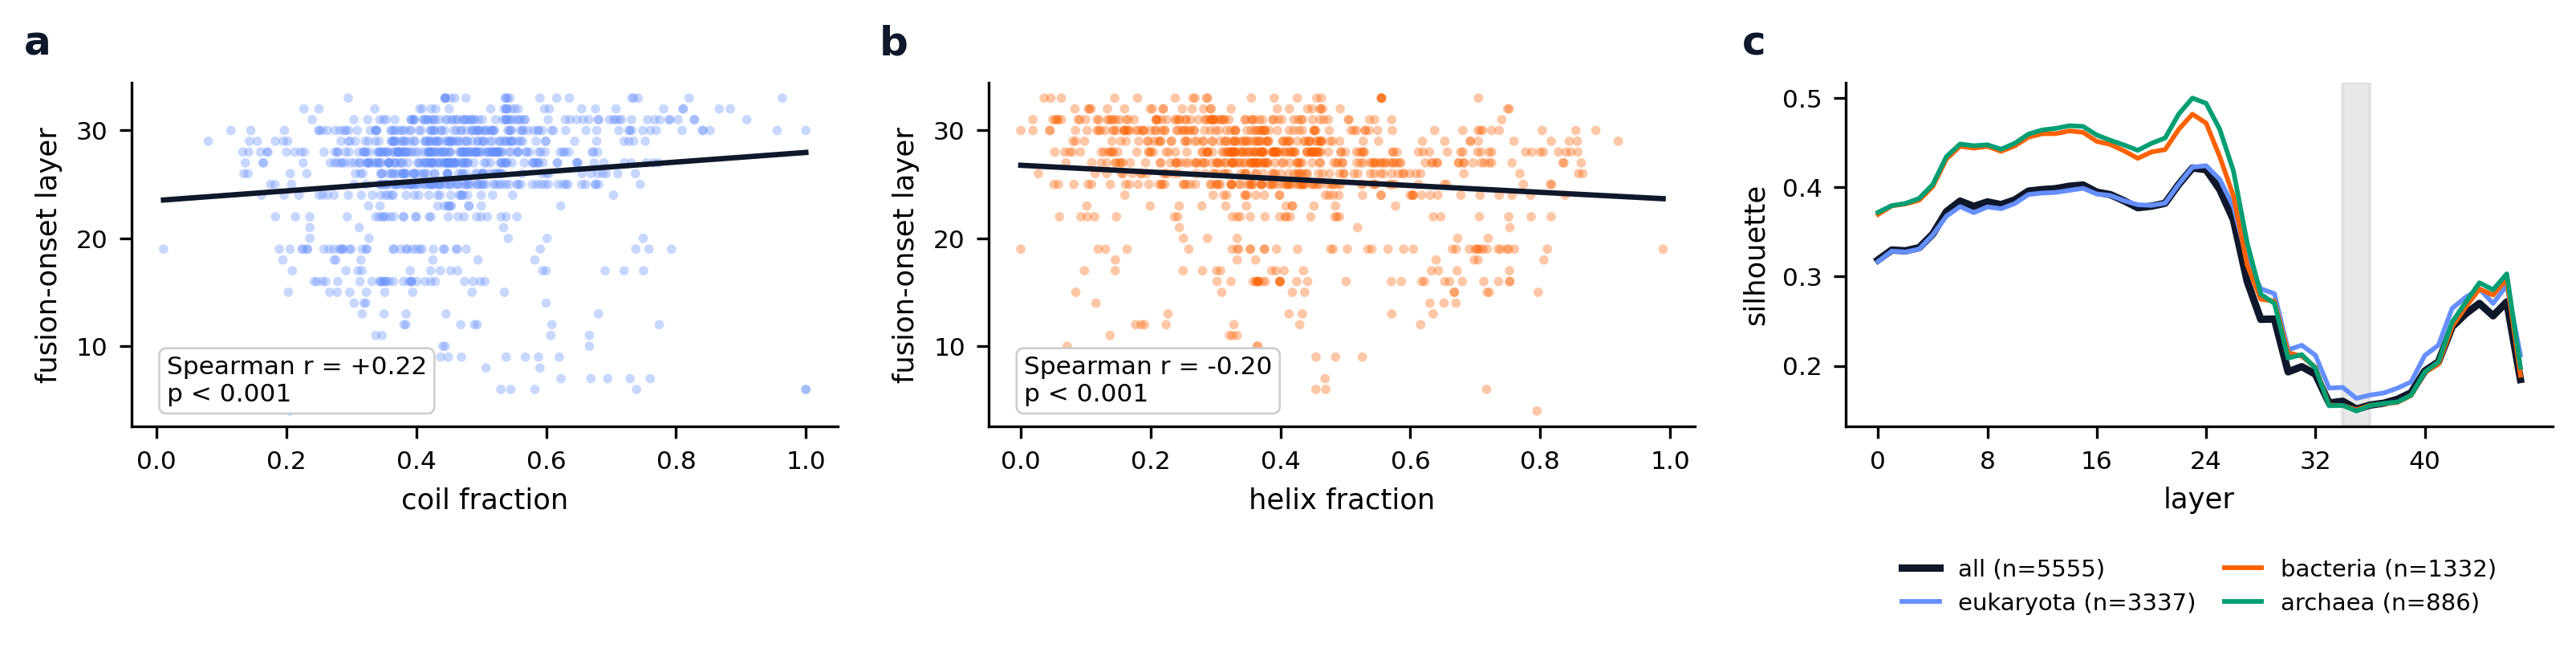
\includegraphics[width=\linewidth]{figure4.png}
\caption{Fusion depth tracks secondary-structure content and is universal across the
tree of life. (a) Per-protein fusion-onset layer averaged within each of ten protein
categories (bars, mean and standard error). Onset is delayed by structural disorder
(Spearman r of $+0.22$ against coil fraction) but is unrelated to protein length
($r = -0.04$, n.s.) or to AlphaFold confidence (mean pLDDT $r = +0.003$, n.s.).
(b) Condition separation across depth for 5,555 proteins from 12 organisms,
stratified by superkingdom. The curves are nearly superimposable and reach minimum
separation at layer 35 (shaded); every one of the 12 organisms reaches its minimum at
layer 35.}
\label{fig:fig4}
\end{figure}

\section{Discussion}

ESM3 organises its inputs into two representational regimes. The four geometry and
sequence modalities collapse into a shared, low-dimensional physical subspace at
mid-depth, whereas the functional-annotation modality occupies a subspace that stays
orthogonal throughout the network. The mid-network timing of physical fusion, the
late entry of sequence, and the dependence of fusion depth on secondary-structure
content together suggest that the network first builds modality-specific features and
then commits to a unified physical representation once secondary structure is
resolved, while holding discrete functional labels on a separate axis. The
depth-locked universality across the tree of life indicates that this organisation is
intrinsic to the trained model rather than a property of any particular proteome.

Geometric orthogonality does not mean that functional content is absent from the
fused representation. A linear probe recovers enzyme class from the structure-derived
representation with a balanced accuracy that rises from 0.56 to about 0.79 by layer
39, and it recovers fold class from the physical conditions at about 0.84 throughout
(Figure S9). The explicit function channel behaves in the opposite way, decoding fold
class only near 0.40 and enzyme class near 0.55, with the latter declining across
depth. The network therefore extracts functional content into the physical subspace
while holding the discrete function channel on a separate and informationally thin
axis, so the orthogonality is a representational choice rather than an absence of
functional information. A causal intervention agrees. Withholding the function input
from the full model displaces the fused representation about six times less than
withholding structure, sequence, or SASA, with a median relative displacement of 0.02
against 0.07 to 0.12 at the fusion layer (Figure S10), so the fused physical
representation is largely insensitive to the function input.

One mechanism that could keep functional annotation orthogonal is redundancy. Because
enzyme class is decodable from the structure-derived representation, the network may
already recover function from the physical modalities and face little pressure to
integrate the explicit functional channel. This account predicts that the function
channel should align more closely with the physical subspace for proteins whose
function is not recoverable from structure. The prediction fails
(Figure S8). Per-protein alignment between the function vector and the
physical subspace is near zero for every protein, with a mean of 0.0005 and a standard
deviation of 0.15, and it does not track redundancy. Proteins for which the structure
representation misclassifies enzyme class align no more strongly than proteins it
classifies correctly, with means of 0.014 and 0.006 and a Mann-Whitney $p$ of 0.35,
and alignment is flat against both the number of InterPro domains, with a Spearman
correlation of $-0.02$, and the number of gene-ontology terms, with a Spearman
correlation of 0.09. Functional annotation therefore stays orthogonal whether or not
it is redundant with the physical modalities, which points away from redundancy and
toward a categorical organisation in which discrete functional labels are held on a
separate axis irrespective of their recoverability from structure.

\section{Limitations}

Several limitations bound these conclusions. Only one model was studied, because
\texttt{esm3-sm-open-v1} is the sole openly available multimodal ESM3, larger ESM3
models are reachable only through a gated interface, and the ESM2 family
\cite{lin2023} is sequence-only and cannot support the experiment. Whether the fractional fusion depth
scales with model capacity therefore remains open. The main structures are AlphaFold
predictions, but the fusion signature is not an artifact of predicted coordinates,
because the disorder effect is uncorrelated with prediction confidence and the
silhouette dip at layer 35, the integration-index rise, and the orthogonality of the
function channel all reproduce on 177 proteins with experimental coordinates
(Figure S11). Finally, the present work
characterises the geometry of the residual stream and does not intervene on it, so
the analysis is descriptive rather than causal.

\section*{Data and code availability}

All analysis code is available at \url{https://github.com/ORGANISATION/REPOSITORY}. The
pipeline is configuration-driven and provides, as separate scripts, dataset curation,
structure retrieval from AlphaFold-DB and the RCSB, secondary-structure and
solvent-accessibility annotation, activation harvesting, the leave-one-out modality
ablation, aggregation, the metric and control analyses, and figure assembly. Random
seeds are fixed throughout.

Representations were extracted from \texttt{esm3-sm-open-v1} \cite{hayes2024}, accessed
through the EvolutionaryScale \texttt{esm} package (version 3.2.1) under its open
licence. The principal dependencies are Python 3.10, PyTorch 2.6, scikit-learn 1.7,
SciPy 1.15, and NumPy 1.26. Secondary structure is computed with DSSP (mkdssp 4.6.1)
\cite{kabsch1983} and solvent accessibility with the Shrake-Rupley implementation
\cite{shrake1973} in ESM's \texttt{ProteinChain}. Figures use the colorblind-safe
\texttt{pypubfigs} palette.

Input data are public. Structure models are from AlphaFold-DB \cite{varadi2022} and
experimental structures from the RCSB, and sequence, InterPro, and Gene Ontology
annotations are from UniProt \cite{uniprot2023,paysanlafosse2023}. Accession lists for
every dataset, including the exact RCSB entries used for the experimental replication,
are provided in the repository. The mean-pooled residual-stream activations, about 24
gigabytes, are regenerated deterministically by the harvesting scripts and are also
deposited at Zenodo (\url{https://doi.org/ZENODO.DOI}).

\bibliographystyle{unsrt}
\bibliography{references}

\end{document}
